\chapter{On the Empirical Likelihood Option Pricing}
\section{Introduction}
Since the seminal works by Black and Scholes (1973) and Merton (1973), option valuation methodologies have been extensively developed. The Black-Scholes model has become one of the most well-known discoveries in the finance literature, which relates the cross-sectional properties of option prices with the underlying asset?returns distribution. However, Rubinstein (1985), Melino and Turnbull (1990) pointed out several limitations in the Black-Scholes model due to the strong assumptions, such as non-normality of the returns, stochastic volatility (implied volatility smile), jumps and others. Both parametric and nonparametric approaches have been proposed to deal with these issues.  

Scott (1987), Hull and White (1987) and Wiggins (1987) extended the Black and Scholes model and allowed the volatility to be stochastic. Heston (1993) developed a closed-form solution for option pricing with the underlying asset volatility being stochastic. Duan (1995) proposed a GARCH option pricing model in an attempt to explain some systematic biases associated with the Black-Scholes model. Later Heston and Nandi (2000) provided a closed-form solution for option pricing with the underlying asset volatility following GARCH(p,q) process. Bates (1996), Bakshi, Cao and Chen (1997) derived an option pricing model with stochastic volatility and jumps. Kou (2002) provided a solution to pricing the option with the double exponential jumps diffusion process. Carr and Madan (1999) introduced the fast Fourier transform approach to option pricing given a specified characteristic function of the return, which provides an efficient computational algorithm to calculate the option prices. For further reference, see Duffie et al. (2000), Bakshi and Madan (2000) and Carr and Madan (2009) among others. All these methods are parametric based, which assume a parametric form of either the distribution of the underlying assets returns or the characteristic function of the underlying assets?returns. 

Nonparametric approaches have also been proposed to capture the underlying asset and option price data to reconstruct the structure of the diffusion process. For example, Hutchinson, Lo and Poggio (1994) applied  neural network techniques to price the derivatives. Ait-Sahalia and Lo (1998) used kernel regression to fit the state-price density implicitly in option pricing. Ait-Sahalia (1996) proposed a nonparametric pricing estimation procedure for interest rate derivative securities under the assumption that the unknown volatility is independent of time. Stutzer (1996) adopted the canonical valuation method, which incorporats the no-arbitrary principle embodied in the formula for calculating the expectation of the discounted value of assets under the risk-neutral probability distribution. 

One of the most important nonparametric methodologies is the empirical likelihood, which conducts likelihood-based statistical inference by profiling a nonparametric likelihood. See Owen (1988, 1990, 2001), DiCiccio and Romano (1989) and Hall and La Scala (1990) for instance. For the application of EL method to time series, see Mykland (1995), Chuang and Chan (2002) and Ling and Chan (2006) among others.  Kitamura (1997) introduced a blockwise empirical likelihood method for weakly dependent time series. Nordman, Sibbertsen and Lahiri (2007) modified the blockwise methods to cope with various dependence structures and achieve better finite sample performance. Yau (2012) studied the application of EL to long-memory time series. 

In this paper, we implement the EL method to price the derivative or options under risk neutral measure. We firstly construct an empirical probability constraint using the historical holding period return time series observations, without assuming the distribution family of the returns. On the other hand, we view the derivative / option price as the parameter of interest directly in the empirical likelihood optimization procedure. An empirical likelihood based estimate of the parameter (e.g. call option price) is obtained and the asymptotic properties of the EL ratio are studied. We further introduce a block-wise empirical likelihood procedure for the weakly dependent processes. Monte Carlo simulation and empirical results for S\&P 500 index option are discussed.     

The remaining of the paper is organized as follows. Section 2 provides a detail empirical likelihood procedure in option pricing. Asymptotic properties are discussed and a robust confidence interval is constructed. Section 3 provides some empirical performance of the empirical likelihood option pricing including both Monte Carlo simulation and S\&P 500 Index options. Section 4 concludes the paper with discussions.

 
\section{Empirical Likelihood on Option Pricing}
Let $P(t)$ be the underlying asset price at time $t$, $D(t)$  the future dividend at time $t$, $r(s,t)$ the gross risk-free interest rate during time $s$ and $t$ with $r(t,t)=1$,  $\mathcal{P}$ the physical probability measure, and $\mathcal{Q}$  the risk-neutral probability measure (See Huang and Litzenberger  (1988)), under which the price process plus the accumulated dividends are martingales after normalization if no arbitrage exists in the pricing systems. To be specific, the latter leads to the following pricing formula.
\begin{eqnarray}
P(t)&=&E^{\mathcal{Q}}[\frac{P(T)+\sum_{s=t}^{T}D(s)r(s,T)}{r(t,T)}]\label{eqn:410}\\
&=&E^{\mathcal{P}}[\frac{P(T)+\sum_{s=t}^{T}D(s)r(s,T)}{r(t,T)}\frac{d\mathcal{Q}}{d\mathcal{P}}].\nonumber
\end{eqnarray}
Here $\frac{d\mathcal{Q}}{d\mathcal{P}}$ is the Radon-Nykodym density of the marginal measure. One can price an option or a derivative security by evaluating the expected discounted value of it under the $\mathcal{Q}$. For example, the call option price with strike price $K$ and expiring date $T$ is given by
\begin{equation}\label{eqn:4102}
C(t,T)=\frac{E ^{\mathcal{Q}}  max[P_T - K,0]   }{r(t,T)} 
\end{equation} 

The following subsection illustrates the idea of estimating $C(t,T)$  through EL coupled with the change-of-measure constraint. 

\subsection{The Estimating Procedure}
Suppose historical data is available in the format of $\{(P(t),D(t)),t=-1,-2,...,-H\}$. A nonparametric way of estimating the option price could be built on approximating $\mathcal{Q}$ by a discrete distribution supported on the observed value of option price, namely $HPR(-i-T,-i)/r(-i-T,-i)$, $1\leq i\leq H-T$ with the corresponding probability denoted by $\pi_i$. Here $HPR(s,t)$ is the holding period return between time $s$ and $t$. If there is no dividend, $HPR(-i-T,i)=P(-i)/P(-i-T)$. Then (\ref{eqn:410}) can be approximated by 

\begin{equation}\label{eqn:4103}
1=\sum_{i=1}^{H-T} \frac{HPR(-i-T,-i)}{r(-i-T,-i)}\pi_i
\end{equation}

Correspondingly, we can estimate the option price by approximating (\ref{eqn:4102}) by
\begin{eqnarray}
\hat{C}(t,T)&=& \sum_{i} \frac{max[P_i(T)-K,0]}{r(t,T)}  \pi_i.
\end{eqnarray}

Note that the choice of $\pi_i$ subjecting to (\ref{eqn:4103}) is not unique. Stutzer (1996) use the idea of maximum entropy, namely maximizing $\sum^{H-T}_{i=1}\pi_ilog\pi_i$ subject to (\ref{eqn:4103}). Here we adopt the Empirical likelihood idea (Owen, 1988) by changing the objective function from entropy to empirical likelihood, namely maximizing $\sum^{H-T}_{i=1}log\pi_i$. Meanwhile, By noticing that the sequence $HPR(-i-T,-i)/r(-i-T,-i)$, $1\leq i\leq H-T$ possesses a reasonable amount of dependence, we suggest  adopting the block wise version of the algorithm as follows. Group the data into $Q$ blocks with with length $M$ is the length of the moving block. Set $L$ to be the step size of the moving block. We obtain block weight $\pi^*_i$ by maximizing $\sum_{i=1}^{H-T} log\pi_i^*$ subject to 
\begin{equation}\label{eqn:4104}
1=\sum_{i=1}^{Q} \pi^*_i \left[\frac{1}{M} \sum_{j=1}^M \frac{HPR(-i*L-j-T, -i*L-j)}{r(-i*L-j-T, -i*L-j)}\right]
\end{equation} 
Then estimate the option price by 
\begin{equation}\label{eqn:4105}
C  =  \sum_{i=1}^Q \frac{max[P_i(T)-K,0]}{r(t,T)}  \pi^*_i
\end{equation} 


This blocking idea has been studied by Kitamura (1997). He argued that using block-wise methods has a much better empirical performance for weakly dependent processes by moving average the noise terms. The estimation procedure in the spirit of Kitamura (1997) would be slightly different, i.e. 
\begin{equation}
max_{C, \pi_i^*} \sum_{i=1}^{Q} log\pi_i^*
\end{equation}
subject to (\ref{eqn:4104}) and  (\ref{eqn:4105}), and the maximizing $C$ will be our estimator. Actually, Peng (2015) has shown that these two approaches yield the same asymptotic property. In our simulation below, we will adopt the second method since it is well known and there is existing package for implementation. Particularly, Qin and Lawless (1994) provided a Lagrangean with multipliers approach to solve the above mentioned optimization problem. We can either apply the numerical optimization process or derive the solution similar to Qin and Lawless (1994). For more details about the Lagrangean optimization or the basic properties of the empirical likelihood procedure, see Owen (1990) and Qin and Lawless (1994). 
  

\subsection{Asymptotic Properties} 
In this subsection, we discuss some basic asymptotic properties of the option price with respect to the empirical likelihood process (Equation (6) / (7)), which helps us to understand the asymptotic distribution of our estimate and conduct further inference.  
\begin{theorem}
Consider 
\[
f(HPR_t,C)=(\frac{max[P_i(T)-K,0]}{r(t,T)}-C, \frac{HPR(-t-T,t)}{r(t-T,t)}-1)^T
\]
and further assume that:\\
(i) the derivative price (C) is in a compact set $\Theta$; \\
(ii) $C_0$ is unique solution of $E(f(HPR_t,C))=0$;\\
(iii) For sufficient small $\delta>0$ and $\eta>0$, 
\[
E[sup_{C^*\in O(C,\delta)}||f(HPR,C^*)||<\infty 
\]
for all $C \in \Theta$;\\
(iv) If a sequence of $C_j$, $j=1,2,...$ converges to some $C$ as $j\rightarrow \infty$, $f(HPR_t,C_j)$ converges to $f(HPR_t,C)$ for all $HPR_t$ except on a null set, which may vary with $C$;\\
(v) $C_0$ is an interior point of $\Theta$;\\
(vi) $Var(H^{-\frac{1}{2}} \sum_{i=1}^H f(HPR_i,C_0))\rightarrow S >0$;\\
(vii) For block-wise empirical likelihood approach, we further assume the weak dependent condition, $\sum_{k=1}^\infty \alpha_X(k)^{1-1/d} <\infty$ for some constant $d>1$. And we require additional assumptions, 
\[
E||f(HPR_t,C_0)||^{2d}<\infty, \text{ for } d>1 
\]  
\[
E sup_{C^* \in O(C_0,\delta)} ||f(HPR_t,C^*)||^{2+\epsilon}<K, \text{ for some }\epsilon>0.
\]
Then, 
\[
LR_0=2\sum_{i=1}^Q log(1+\gamma(\hat{C})^T f(HPR_i,\hat{C})) \rightarrow_{dist.}  \chi _1^2
\]
\end{theorem}
where $K$ is a finite number, $\gamma(\hat{C})$ is the Lagrange multiplier vector and $Q$ is the total number of states. Particularly for non-blockwise empirical likelihood case (i.e. Equation (6)), $Q=H-T$.

Theorem 1 provides an asymptotic distribution of the likelihood ratio $LR_0$, which can be further applied to inference of the estimate. We omit the detailed proof here.\footnote{Our proof is based on Theorems 1 \& 2 in Kitamura (1997). } For independent observations of $HPR_i$, we only require the assumptions (i)-(vi) to have the asymptotic property of the likelihood ratio; and for weak-dependent observations of $HPR_i$, assumption (vii) is additionally required. 




\section{Empirical Results}
In this section,  we will first compare our method with Black-Scholes model through simulation and then conduct an empirical analysis on the option pricing for the S\&P 500 index call options.  

\subsection{Monte Carlo Simulation}

Following Hutchinson et al. (1994), Ait-Sahalia and Lo (1995) and  Stutzer (1996), we generate a geometric Brownian motion process with a 10 percent drift and 20 percent annualized volatility. Firstly we simulated 2 years of historical daily stock returns with $253\times 2=506$ observations. We repeat 200 samples, and for each sample, three different prices are calculated. 1. the estimated price by the empirical likelihood option pricing procedure; 2. the estimated price by the Black-Scholes model with historical volatility; 3. the actual price by the Black-Scholes model with actual volatility. The performance of the first two prices are compared based on the mean absolute percentage error (MAPE) with respective to the third price, which is considered to be minicing the true price. The comparison is make at different price-to-strike price ratios (i.e. $P/X=\frac{9}{10}, 1, \frac{9}{8}$) and different expiration dates (i.e. $T=\frac{1}{13}, \frac{1}{4}, \frac{1}{2}$). 


\begin{center}
[Table 1]
\end{center}

Table 1 provides the simulation performance: Panel A reports the MAPE of the empirical likelihood (EL) option price, and Panel B reports the MAPE of the historical volatility based Black Scholes price. In the perfect Black-Scholes world, the Black-Scholes formula using the historical volatility outperforms the empirical likelihood option pricing methodology. This is because the Black-Scholes formula only requires the second moment information and $506$ observations can provide a very good estimate of the second moment, but  empirical likelihood method will automatically capture the higher order moment information, which will not benefit in pricing the options in the perfect Black-Scholes world.  

We are also interested in the accuracy of the empirical likelihood option pricing for different moneyness and days-to-maturity. The empirical likelihood option pricing method provides very good performance in pricing the in-the-money options with small MAPE. However, the MAPE are very significant for out-of-the-money options. At-the-money option pricing error is in between. On the other hand, the pricing errors have different patterns for in-the-money, at-the-money and out-of-the-money options. For in-the-money and at-the-money options, the fewer days to maturity, the smaller pricing errors are. For out-of-the-money option, the fewest days to maturity case has the largest pricing error, with a possible reason that the price magnitude of the out-of-the-money options with very few days to maturity is already very small.  

\subsection{S\&P 500 Index Options}

We also implement the empirical likelihood option pricing method in pricing the S\&P 500 index options. The daily return data is from Center for Research in Security Prices (CRSP) and the option data is from OptionMetrics. The daily return data is from Jan 2011 to Dec 2012. We use the year 2011 daily return data as the formation period, and then test its performance in the year 2012 daily index options pricing comparing with the historical volatility based Black Scholes model and the true values. We only keep the options which have the Moneyness closest to 1 and days to maturity between 15 to 50. 
\begin{center}
[Figure 1]
\end{center}

Figure 1 shows the time series of the option prices. The red line is true value of the market daily close price, the green line is the empirical likelihood option price and the blue line is the Black Scholes option price using the historical volatility. Due to the stock price movement, the true option prices vary from 1.5 to 3.7. However, the historical volatility based Black Scholes option prices are consistently overpriced for the at-the-money call options, as is documented in Hull and White (1987).  the contrast, our EL option prices are a lot closer to the true option market prices. This is because our empirical likelihood methodology also captures the high order moment information, while the historical volatility based Black Scholes option model only captures the second moment information.   


\section{Conclusion}
In this paper, we introduce an empirical likelihood method to price the derivatives or options under risk-neutral measure $\mathcal{Q}$. Monte Carlo simulations show that our new pricing methodology performs reasonably well for the at-the-money and in-the-money options. We also apply our empirical likelihood option pricing method to S\&P 500 index options, and the results demonstrate that our method outperforms the historical volatility based Black Scholes model. This is due to the advantage of EL method in capturing the high order moment information.

\begin{table}[t]
\centering \caption{ Monte Carlo Simulation in a Black-Scholes Market}

\begin{quote} %\linespread{1.8} \selectfont

This table reports the mean absolute percentage error (MAPE) of the empirical likelihood (EL) option price to the ideal Black-Scholes price (Panel A), the historical volatility based Black Scholes price to the ideal Black-Scholes price (Panel B) for different combination of the relative exercise prices ($P/K$) and time to expiration date. The price dynamics follow the Geometric Brownian Motion with $\mu=0.1$ and $\sigma=0.2$. The relative exercise prices ($P/K$) are chosen as Rubinstein (1985), Stutzer (1996). The time to expiration date are $1/13, 1/4, 1/2$ years, respectively.  
\end{quote}

\begin{tabular}{ccccc}
\noindent Panel A: &&&& \\

\hline\hline 
& Hist Var vs Ideal BS & & Days to Maturity &\tabularnewline
& & 1/13 & 1/4 & 1/2\tabularnewline
\hline 

& 9/10 & 0.139 & 0.066 & 0.046\tabularnewline

Moneyness ($P/K$) & 1 & 0.022 & 0.020 & 0.019\tabularnewline

& 9/8 & 0.000 & 0.003 & 0.005\tabularnewline \hline
\end{tabular}\newline\newline\newline


\begin{tabular}{ccccc}
\noindent Panel B: &&&& \\
\hline\hline 
& EL vs Ideal BS & & Days to Maturity &\tabularnewline
& & 1/13 & 1/4 & 1/2\tabularnewline
\hline 

& 9/10 & 0.724 & 0.514 & 0.537\tabularnewline

Moneyness ($P/K$) & 1 & 0.088 & 0.149 & 0.230\tabularnewline

& 9/8 & 0.003 & 0.025 & 0.058\tabularnewline \hline
\end{tabular}\newline

\end{table}

\newpage

\begin{figure}[t]
\centering \caption{Comparison of the S\&P 500 index option prices and EL option prices}

\begin{quote} %\linespread{1.8} \selectfont

This figure shows the time series of three S\&P 500 index option prices. We only keep the options have the Moneyness closest to 1 and days to maturity between 15 to 50. The red line is true value of the market daily close price, the green line is the empirical likelihood option price and the blue line is the Black Scholes option price using the historical volatility. 
\end{quote}
  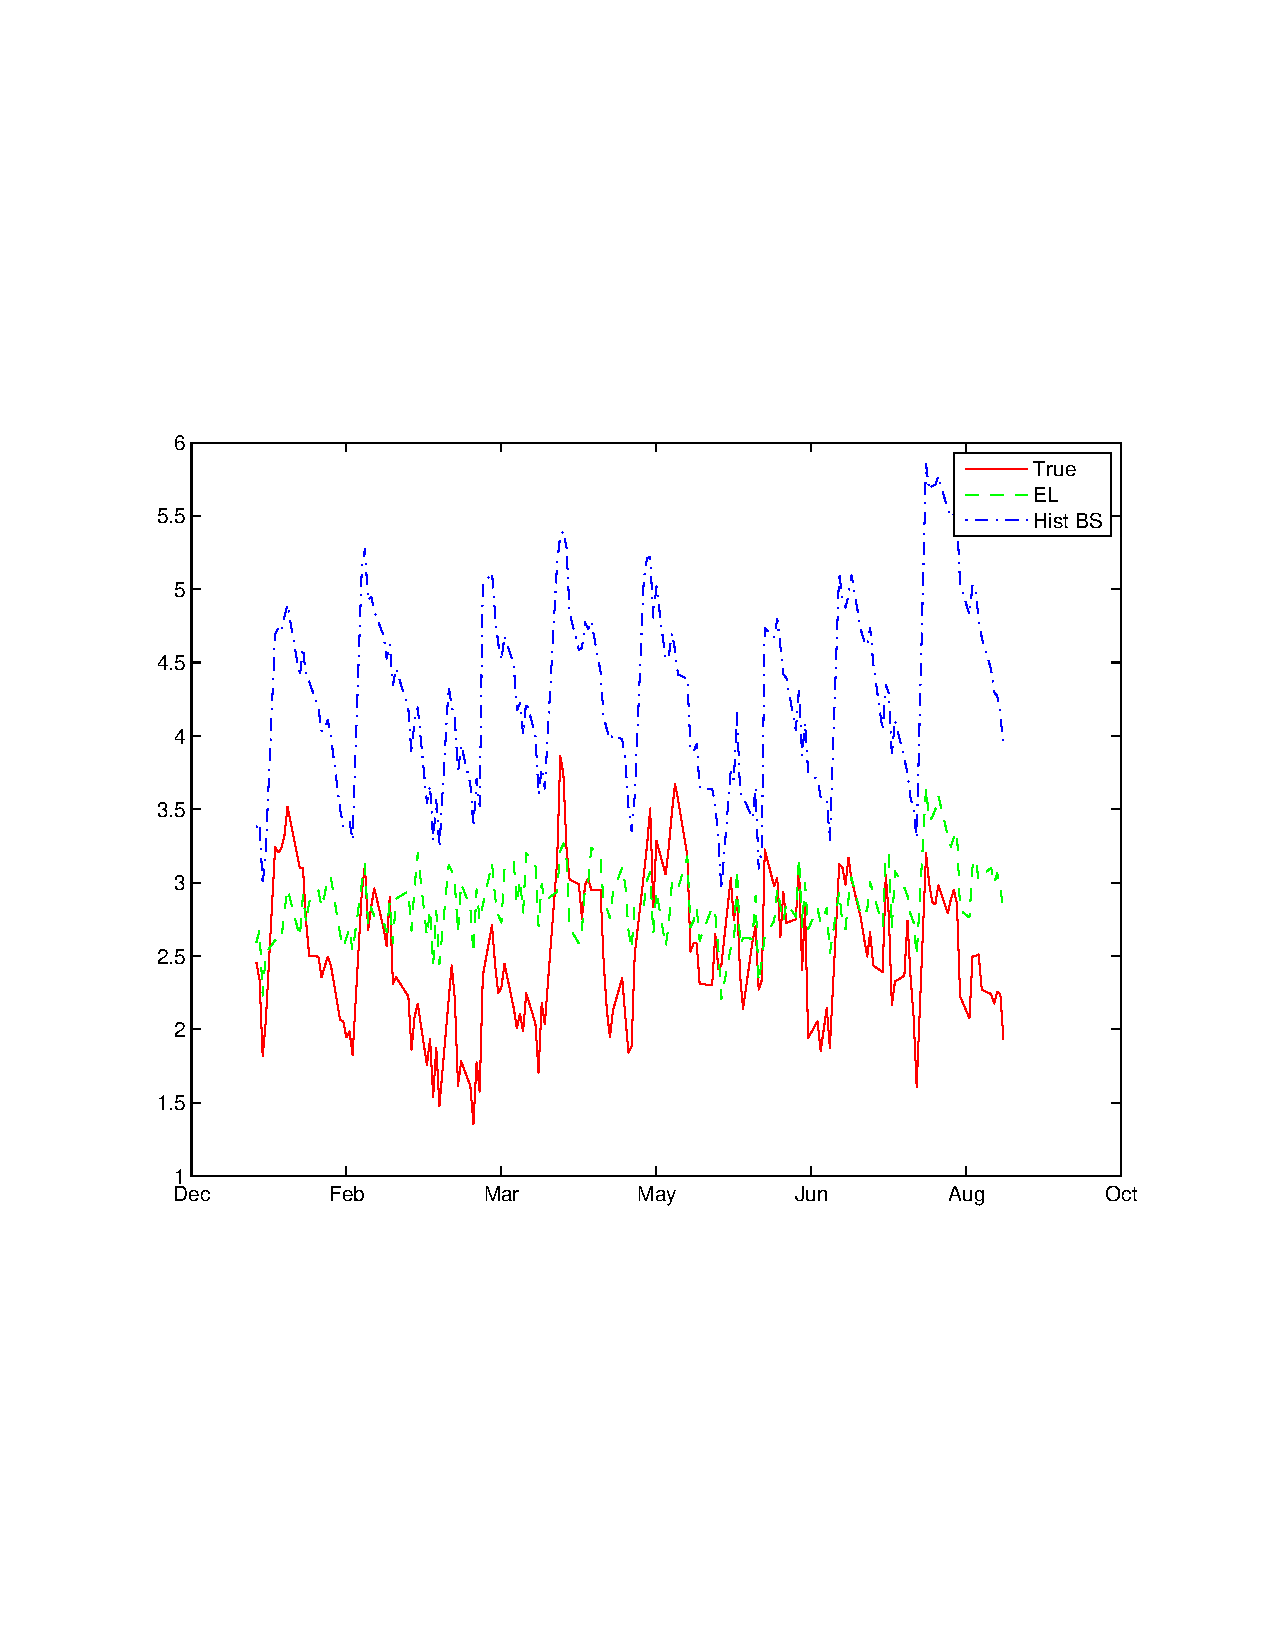
\includegraphics[width=0.8\textwidth]{SP500.pdf}
\end{figure}

